% Propostas para substituir o Quadro 3 "Configurações testadas na otimização"
% (05/11/2026, pedido do autor). NÃO é parte do TG. Valores conferidos em
% dados/resultados/refeito_2026-10-05/grades/r3_*.txt.
\documentclass[11pt,a4paper]{article}
\usepackage[T1]{fontenc}
\usepackage[brazilian]{babel}
\usepackage{mathptmx}
\usepackage[a4paper,margin=2.4cm]{geometry}
\usepackage{graphicx}
\usepackage[font=small,labelfont=bf]{caption}
\usepackage[most]{tcolorbox}
\usepackage[hidelinks]{hyperref}
\setlength{\parskip}{0.45em}
\setlength{\parindent}{0pt}

\definecolor{cesc}{RGB}{220,50,32}
\definecolor{cmod}{RGB}{0,90,181}
\newtcolorbox{ideia}[1][]{colback=cmod!5, colframe=cmod!70, fonttitle=\bfseries, title={#1}, arc=2pt, boxrule=0.6pt}
\newtcolorbox{cuidado}[1][]{colback=cesc!4, colframe=cesc!70, fonttitle=\bfseries, title={#1}, arc=2pt, boxrule=0.6pt}

\title{Alternativas ao Quadro 3\\[2pt]\large configurações testadas na otimização}
\author{Material de análise, fora do TG}
\date{5 de novembro de 2026}

\begin{document}
\maketitle

O Quadro~3 lista as seis formas de uso do GARCH, os valores testados de cada
parâmetro e a conta que leva às 312 configurações. Ele é completo, mas a conta
($8 \times 3 \times 2 \times 2$) obriga o leitor a montar a grade de cabeça. Este
relatório traz duas formas de desenhar a mesma informação. Nada aqui foi colocado
no \texttt{tg/}.

\section{Proposta A: a grade desenhada}

\begin{figure}[h]
\centering
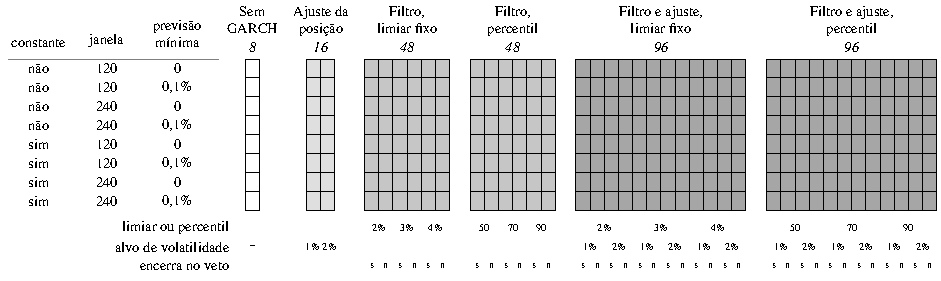
\includegraphics[width=\textwidth]{fig-grade-blocos.pdf}
\caption{Cada quadrado é uma das 312 configurações simuladas}
\end{figure}

Cada quadrado é uma simulação. As oito linhas são as combinações que todas as
formas compartilham: com ou sem constante, janela de 120 ou 240 pregões e
previsão mínima de zero ou 0,1\%. Cada coluna é uma combinação dos parâmetros
próprios da forma de uso, lida embaixo dela (``s'' e ``n'' são sim e não para
encerrar a posição no veto). Contar os quadrados de um bloco dá o número do
Quadro~3, e todos os blocos juntos dão $39 \times 8 = 312$.

\begin{ideia}[O que essa forma mostra melhor]
De onde vem cada número: o 8 é a altura, igual para todos, e o resto é a largura
de cada bloco. Também fica visível, sem conta, que as duas formas que combinam
filtro e ajuste da posição respondem por quase dois terços da grade.
\end{ideia}

\begin{cuidado}[Pontos fracos]
É uma figura densa, com letra pequena nos rótulos de baixo. No TG ela ocuparia a
largura toda da página e precisaria de uma nota explicando ``s'' e ``n''.
\end{cuidado}

\section{Proposta B: gráfico de barras}

\begin{figure}[h]
\centering
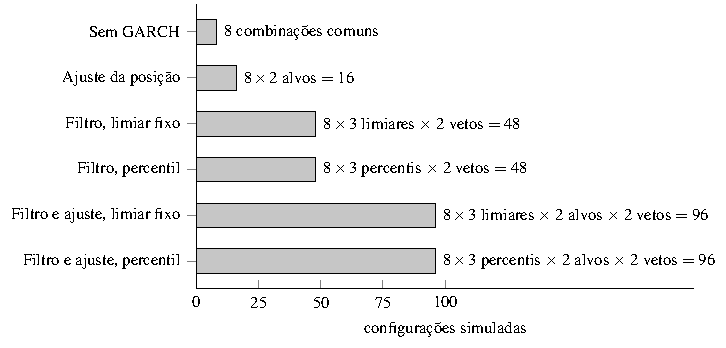
\includegraphics{fig-grade-barras.pdf}
\caption{Número de configurações de cada forma de uso do GARCH}
\end{figure}

Cada barra é uma forma de uso, com o tamanho proporcional ao número de
configurações e a conta escrita ao lado. É a leitura mais rápida: bate o olho e
vê quais formas pesaram mais na otimização.

\begin{cuidado}[Pontos fracos]
A barra mostra quantos, mas não quais. Os valores testados (limiar de 2\%, 3\% ou
4\%, percentil 50, 70 ou 90, alvo de 1\% ou 2\%) somem do desenho e teriam de ir
para o texto ou para uma nota. Pela norma seria um Gráfico, não uma Figura.
\end{cuidado}

\section{Comparação e recomendação}

A proposta A substitui o Quadro~3 por inteiro, porque mostra os valores e a conta
ao mesmo tempo. A proposta B é mais simples de ler, mas só substitui o quadro se
os valores dos parâmetros forem para o texto. A recomendação é a A. A B serve se a
ideia for complementar o quadro em vez de substituí-lo.

\begin{cuidado}[O que mudaria no TG]
Com a linha do tempo dos períodos, o TG já tem 4 quadros e lista única de
ilustrações. Trocar o Quadro~3 por figura deixa 3 quadros, sem nenhuma mudança
nova nas listas. O texto do Capítulo~II que cita o quadro (``como mostra o
Quadro~3'') passaria a citar a figura, e a nota do quadro sobre o número 8 fica
desnecessária na proposta A, porque as oito linhas estão desenhadas.
\end{cuidado}
\end{document}
